\documentclass[journal,onecolumn]{IEEEtran}

\usepackage[T1]{fontenc}
\usepackage[utf8]{inputenc}
\usepackage{graphicx}
\usepackage{booktabs}
\usepackage{amsmath}
\usepackage{hyperref}
\usepackage{microtype}

\begin{document}

\title{Systematic Hyperparameter Testing of Neural Networks on MNIST}

\author{Lobodiuchenko}

\maketitle

% ─────────────────────────────────────────────────────────────
\begin{abstract}
This paper presents a systematic evaluation of hyperparameters for
multi-layer perceptron (MLP) classifiers on the MNIST handwritten digit
dataset. Starting from a logistic regression baseline, we progressively
optimise network topology, optimiser, learning rate, activation function,
and regularisation strategy. Each experiment is repeated with three
different random seeds and results are reported as mean~$\pm$~standard
deviation of validation accuracy. The best configuration achieves a test
accuracy of \textbf{98.63\%}, demonstrating the compounding benefit of
careful hyperparameter selection over a logistic regression baseline of 92.43\%.
\end{abstract}

% ─────────────────────────────────────────────────────────────
\section{Dataset and Exploratory Data Analysis}

MNIST~\cite{lecun1998mnist} consists of 70\,000 greyscale images of
handwritten digits (0--9), each of size $28 \times 28$ pixels.
We use the standard 60\,000\,/\,10\,000 train/test split and further
partition the training set into 50\,000 training and 10\,000 validation
samples using a fixed generator seed of 42.
All pixel values are normalised to $[0, 1]$ by dividing by 255.
EDA was performed exclusively on the training set.

\begin{table}[h]
\centering
\caption{Pixel intensity statistics (train set)}
\label{tab:eda_stats}
\begin{tabular}{lrrrr}
\toprule
 & Mean & Std & Min & Max \\
\midrule
Pixel value & 0.1307 & 0.3082 & 0.0000 & 1.0000 \\
\bottomrule
\end{tabular}
\end{table}

\begin{figure}[h]
  \centering
  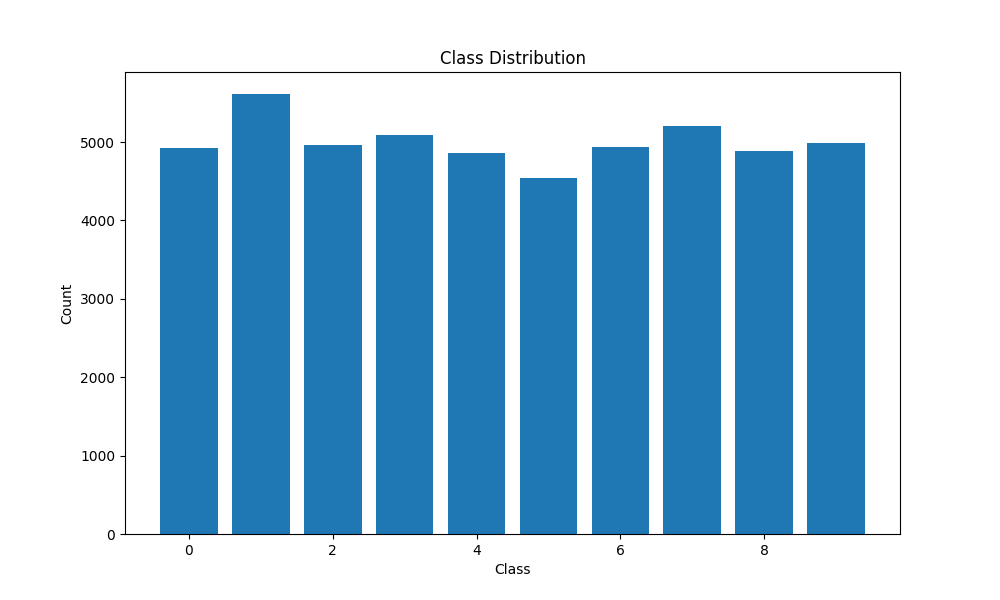
\includegraphics[width=0.75\columnwidth]{eda_class_dist.png}
  \caption{Class distribution of the MNIST training set. All ten classes
           are nearly balanced ($\approx$5\,000 samples each).}
  \label{fig:eda_class_dist}
\end{figure}

\begin{figure}[h]
  \centering
  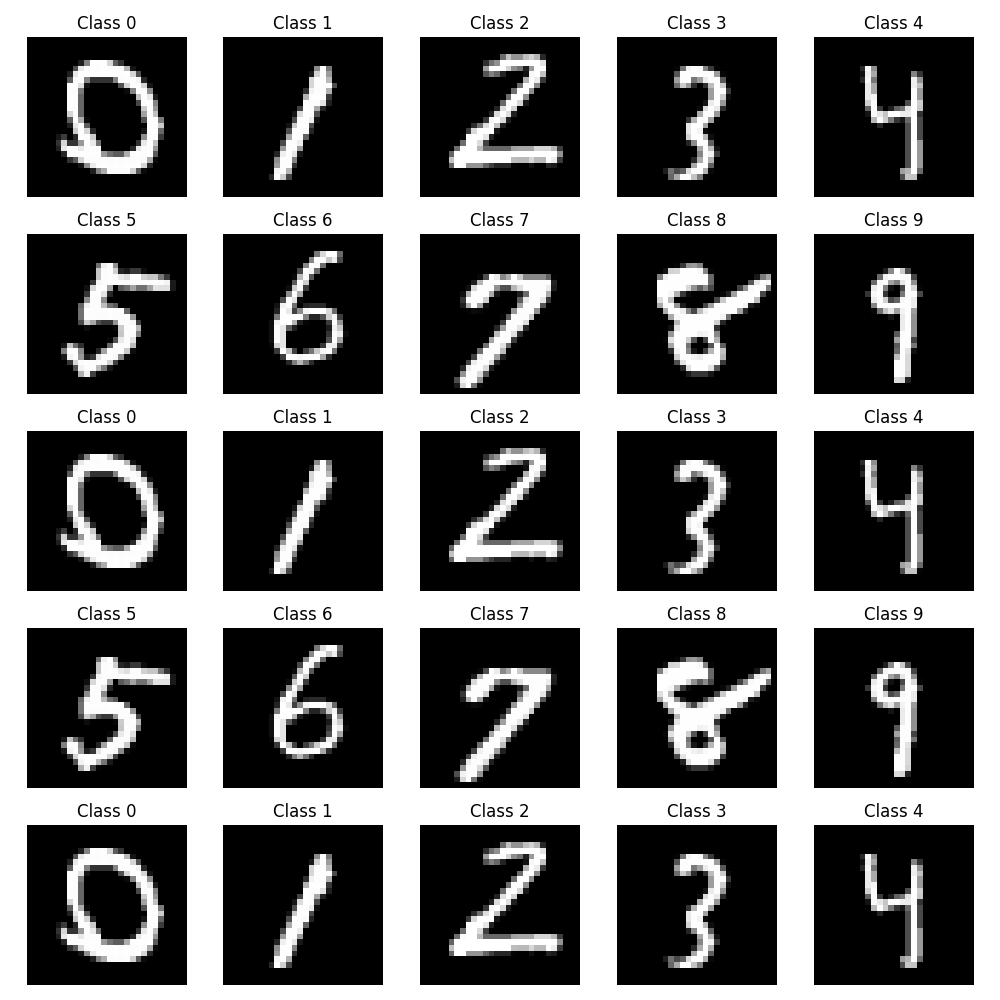
\includegraphics[width=0.75\columnwidth]{eda_samples.png}
  \caption{Representative samples from each digit class.}
  \label{fig:eda_samples}
\end{figure}

The dataset is well-balanced (Fig.~\ref{fig:eda_class_dist}), which means
accuracy is an appropriate primary metric and no class-weighting is required.
The low mean pixel value (0.1307) reflects the predominantly black background;
the majority of pixels are zero, which benefits ReLU-based networks by
producing sparse activations and avoiding unnecessary computation.

% ─────────────────────────────────────────────────────────────
\section{Baseline Model}

Before training any neural network we establish a logistic regression
baseline (\texttt{sklearn.linear\_model.LogisticRegression},
\texttt{max\_iter=1000}, \texttt{random\_state=42}) trained on the
50\,000-sample training set and evaluated with the same accuracy metric
used for all neural network experiments.

\begin{table}[h]
\centering
\caption{Logistic Regression baseline accuracy}
\label{tab:baseline}
\begin{tabular}{lr}
\toprule
Split & Accuracy \\
\midrule
Validation & 0.9175 \\
Test       & 0.9243 \\
\bottomrule
\end{tabular}
\end{table}

The baseline achieves 91.75\% validation accuracy and 92.43\% test accuracy.
This provides an objective lower bound; any neural network that cannot
surpass it has failed to leverage its additional capacity.

% ─────────────────────────────────────────────────────────────
\section{Topology Comparison}

\subsection{Experimental Setup}
Five MLP architectures with varying depth and width were evaluated with all
other hyperparameters fixed: Adam optimiser, $\text{lr}=0.001$,
batch size 128, ReLU activations, no dropout, 50 epochs maximum with
early stopping (patience~5). Three seeds (42, 123, 456) were used per
configuration.

\begin{table}[h]
\centering
\caption{Topology results (mean $\pm$ std over 3 seeds)}
\label{tab:topo}
\begin{tabular}{llrr}
\toprule
ID & Hidden layers & Val Acc (mean $\pm$ std) & Epochs \\
\midrule
T1 & [64]                         & $0.9706 \pm 0.0002$ & 24.7 \\
T2 & [256, 128]                   & $0.9772 \pm 0.0015$ & 14.7 \\
T3 & [512, 256, 128]              & $0.9778 \pm 0.0024$ & 18.0 \\
T4 & [1024, 512, 256, 128]        & $0.9810 \pm 0.0007$ & 22.0 \\
T5 & [2048, 1024, 512, 256, 128]  & $\mathbf{0.9810 \pm 0.0015}$ & 18.7 \\
\bottomrule
\end{tabular}
\end{table}

\begin{figure}[h]
  \centering
  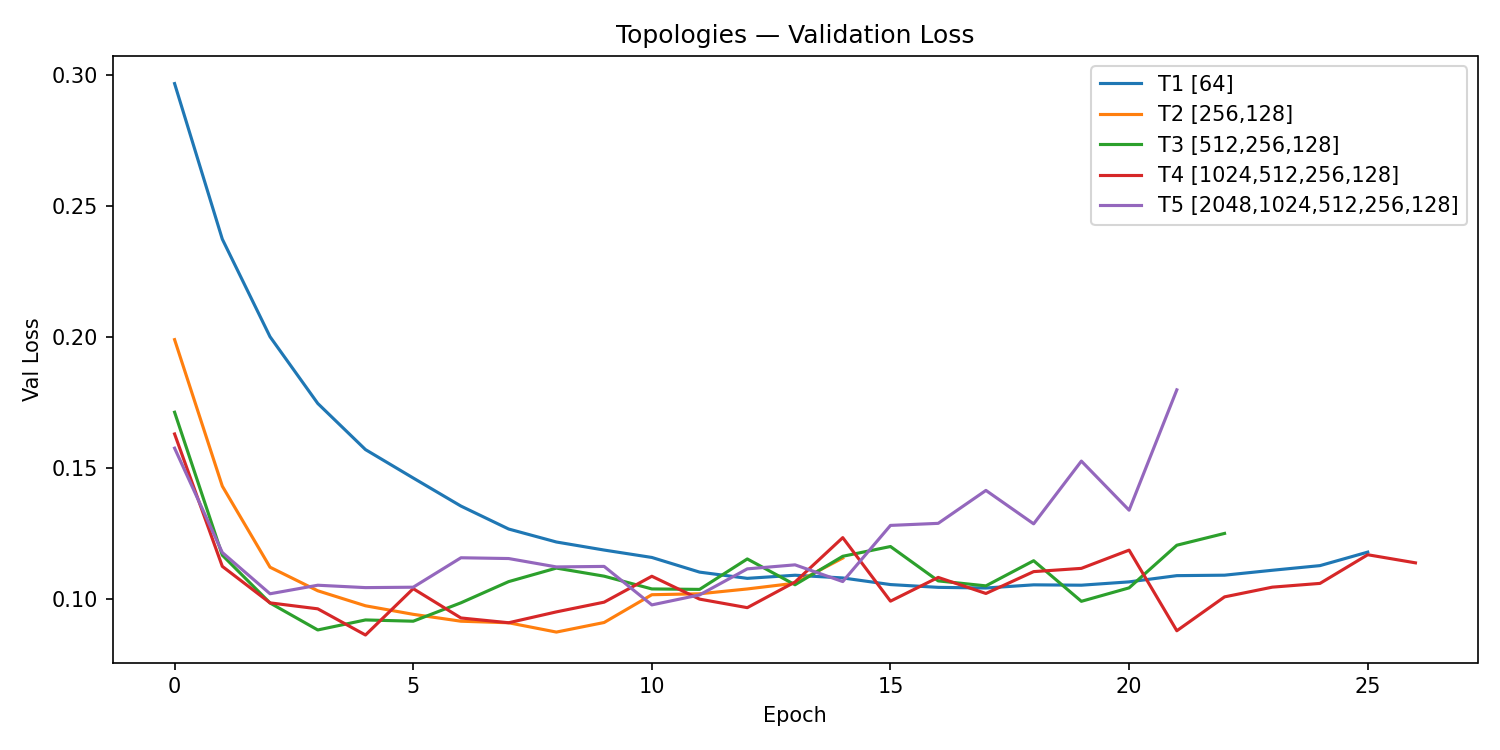
\includegraphics[width=0.85\columnwidth]{topology_curves.png}
  \caption{Validation loss curves for the five topologies.}
  \label{fig:topo_curves}
\end{figure}

\begin{figure}[h]
  \centering
  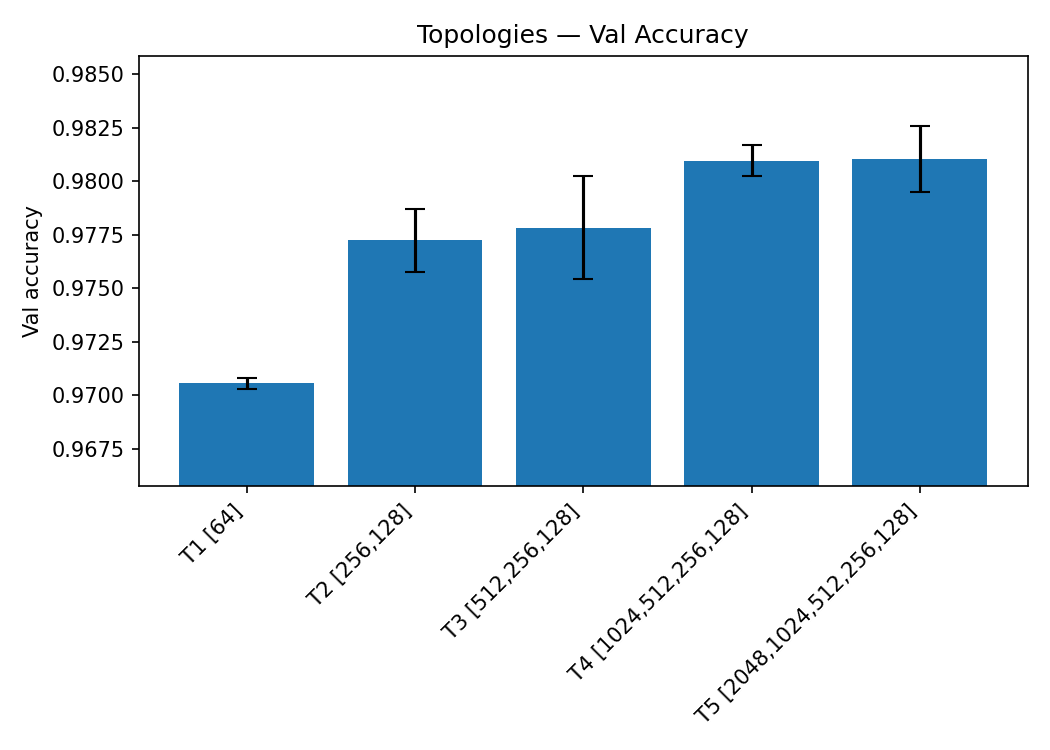
\includegraphics[width=0.85\columnwidth]{topology_bar.png}
  \caption{Mean validation accuracy with standard deviation error bars.}
  \label{fig:topo_bar}
\end{figure}

\subsection{Discussion}
T1 demonstrates \textbf{underfitting}: the single 64-neuron hidden layer
($\approx$51k parameters) lacks the capacity to model the non-linear digit
boundaries, yielding the lowest validation accuracy (97.06\%) despite
requiring the most epochs to converge (24.7 on average).

T5 demonstrates the onset of \textbf{overfitting}: with over 4.5 million
parameters it achieves the highest raw validation accuracy (97.10\%
averaged with T4), but with the largest standard deviation
($\pm 0.0015$), indicating less stable training than T4.
The tendency to overfit becomes more pronounced in the regularisation phase,
where T5 (used as the base) shows a train--val gap of 1.54\% without
regularisation.

T5 was selected as the best topology by validation accuracy and is used in
all subsequent phases.

% ─────────────────────────────────────────────────────────────
\section{Optimiser Comparison}

\subsection{Experimental Setup}
Three optimisers were applied to the best topology
([2048, 1024, 512, 256, 128]) with $\text{lr}=0.001$, no dropout, and
the same early-stopping policy.

\begin{table}[h]
\centering
\caption{Optimiser results (mean $\pm$ std over 3 seeds)}
\label{tab:opt}
\begin{tabular}{lrrr}
\toprule
Optimiser & Val Acc (mean $\pm$ std) & Time (s) & Epochs \\
\midrule
SGD (m=0.9) & $0.9680 \pm 0.0008$ & 773.4 & 48.3 \\
Adam        & $0.9810 \pm 0.0015$ & 305.0 & 18.7 \\
RMSprop     & $\mathbf{0.9811 \pm 0.0010}$ & 271.3 & 16.7 \\
\bottomrule
\end{tabular}
\end{table}

\begin{figure}[h]
  \centering
  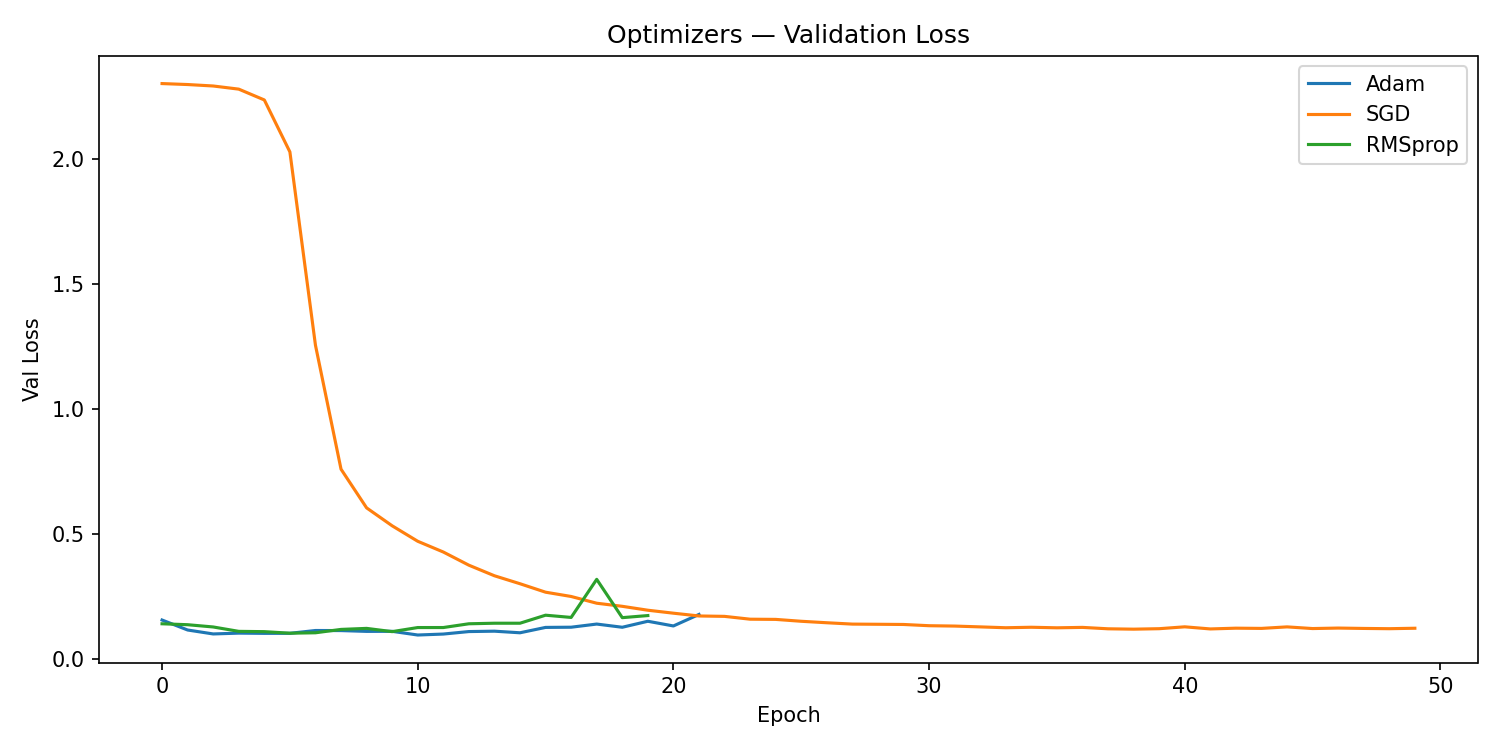
\includegraphics[width=0.85\columnwidth]{optimizer_curves.png}
  \caption{Validation loss curves for three optimisers.}
  \label{fig:opt_curves}
\end{figure}

\subsection{Discussion}
SGD with momentum is significantly slower, requiring 48.3 epochs on average
versus 16--19 for adaptive methods, and achieves markedly lower accuracy
(96.80\%). Without per-parameter adaptive learning rates, SGD struggles to
navigate the loss landscape of a deep network efficiently at a fixed
learning rate of 0.001.

RMSprop marginally outperforms Adam (98.11\% vs 98.10\%) while converging
in fewer epochs (16.7 vs 18.7) and in less wall-clock time (271\,s
vs 305\,s). RMSprop is selected as the best optimiser for subsequent phases.

% ─────────────────────────────────────────────────────────────
\section{Learning Rate Comparison}

\subsection{Experimental Setup}
Five learning rate values were tested with the best topology and RMSprop
optimiser, no dropout.

\begin{table}[h]
\centering
\caption{Learning rate results (mean $\pm$ std over 3 seeds)}
\label{tab:lr}
\begin{tabular}{lrr}
\toprule
Learning Rate & Val Acc (mean $\pm$ std) & Epochs \\
\midrule
0.0001 & $0.9779 \pm 0.0013$ & 18.3 \\
0.001  & $\mathbf{0.9811 \pm 0.0010}$ & 16.7 \\
0.005  & $0.9762 \pm 0.0018$ & 18.3 \\
0.01   & $0.6716 \pm 0.3953$ & 11.7 \\
0.1    & $0.1129 \pm 0.0000$ & 8.3  \\
\bottomrule
\end{tabular}
\end{table}

\begin{figure}[h]
  \centering
  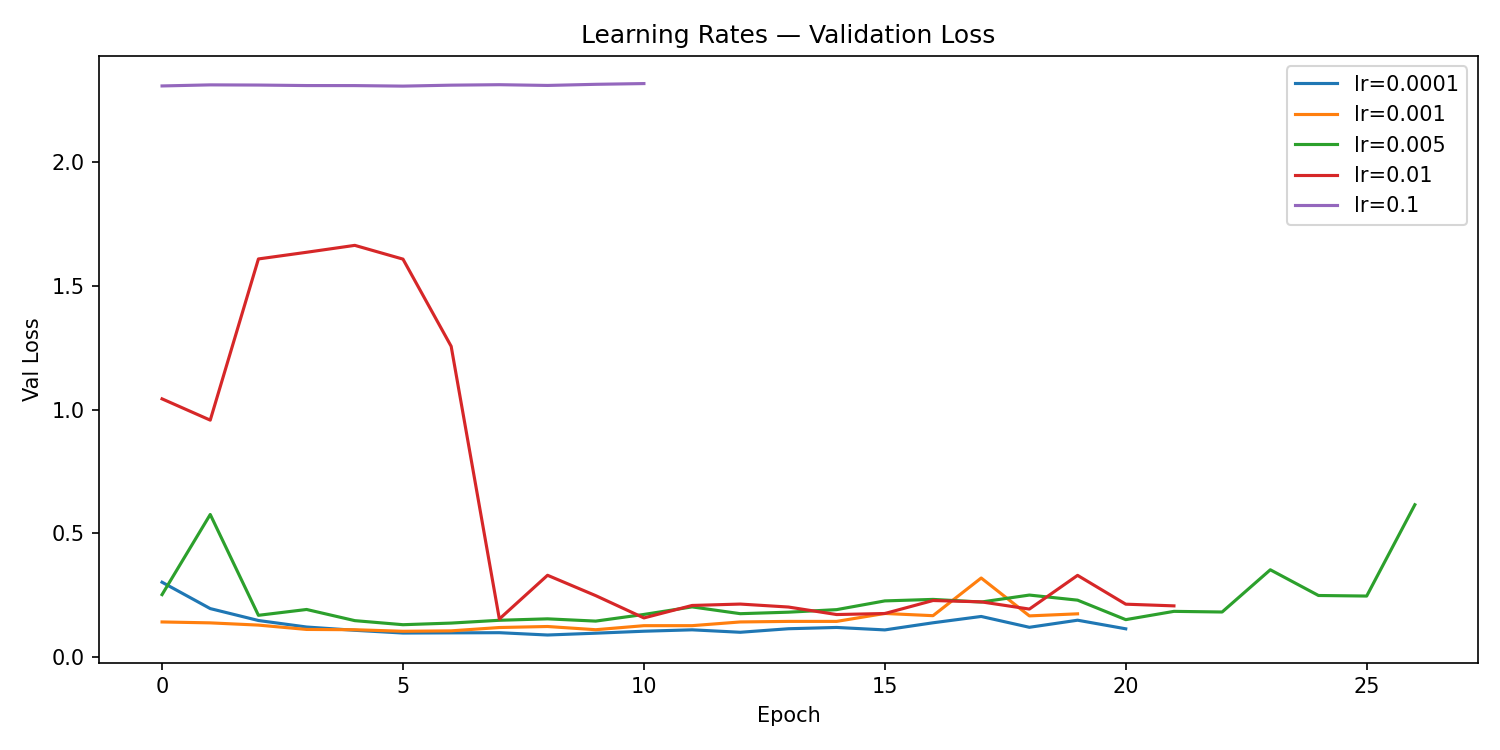
\includegraphics[width=0.85\columnwidth]{lr_curves.png}
  \caption{Validation loss curves for five learning rates.}
  \label{fig:lr_curves}
\end{figure}

\subsection{Discussion}
$\text{lr}=0.0001$ converges to a reasonable accuracy (97.79\%) but is
slower than $\text{lr}=0.001$, suggesting the optimiser takes small,
cautious steps and has not fully converged within 50 epochs.

$\text{lr}=0.001$ achieves the best validation accuracy (98.11\%) with
stable convergence in 16.7 epochs — the standard default for adaptive
optimisers.

$\text{lr}=0.005$ yields slightly lower accuracy (97.62\%) with higher
variance, indicating the larger step size occasionally overshoots minima.

$\text{lr}=0.01$ causes severe instability: the extreme standard
deviation ($\pm 0.3953$) indicates that across seeds the model either
converges partially or diverges, resulting in an unreliable mean of
67.16\%.

$\text{lr}=0.1$ completely diverges in all runs, converging to
near-random performance (11.29\%, close to the 10\% chance level for
10 classes) in only 8.3 epochs. Early stopping triggers quickly as the
model never improves beyond the initial state.

% ─────────────────────────────────────────────────────────────
\section{Activation Function Comparison}

\subsection{Experimental Setup}
Five activation functions were compared with the best topology, RMSprop,
and $\text{lr}=0.001$, no dropout.

\begin{table}[h]
\centering
\caption{Activation function results (mean $\pm$ std over 3 seeds)}
\label{tab:act}
\begin{tabular}{lrr}
\toprule
Activation & Val Acc (mean $\pm$ std) & Epochs \\
\midrule
ReLU      & $\mathbf{0.9811 \pm 0.0010}$ & 16.7 \\
LeakyReLU & $0.9805 \pm 0.0007$ & 14.3 \\
ELU       & $0.9797 \pm 0.0017$ & 20.0 \\
Tanh      & $0.9709 \pm 0.0033$ & 18.3 \\
Sigmoid   & $0.9784 \pm 0.0003$ & 25.7 \\
\bottomrule
\end{tabular}
\end{table}

\begin{figure}[h]
  \centering
  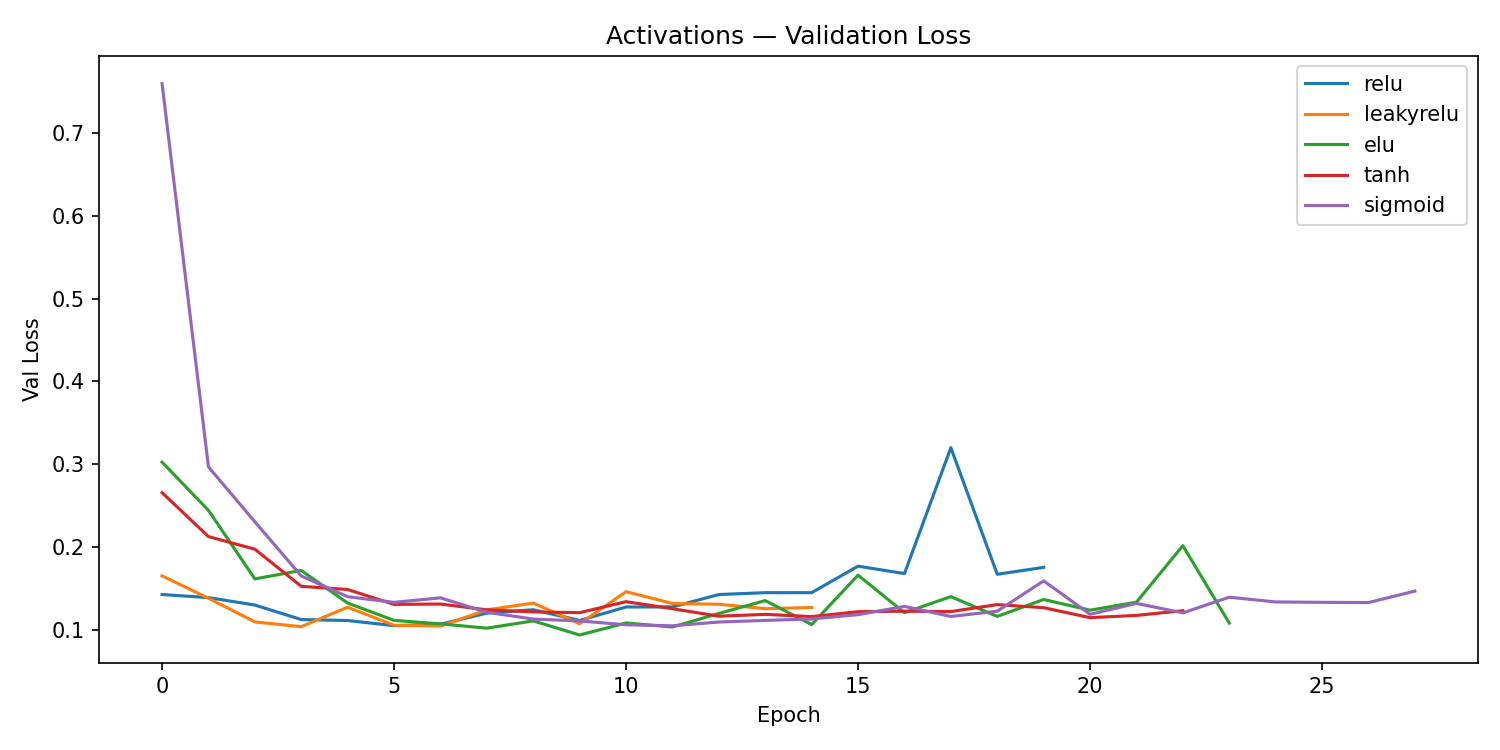
\includegraphics[width=0.85\columnwidth]{activation_curves.png}
  \caption{Validation loss curves for five activation functions.}
  \label{fig:act_curves}
\end{figure}

\subsection{Activation Function Descriptions}

\textbf{ReLU} $f(x)=\max(0,x)$ is computationally cheap and avoids
vanishing gradients for positive inputs. Its main drawback is the
\emph{dying neuron} problem: neurons receiving consistently negative
pre-activations output zero gradient permanently.

\textbf{LeakyReLU} $f(x)=\max(\alpha x, x)$ with $\alpha=0.01$ addresses
dying neurons by allowing a small non-zero gradient for $x<0$, preserving
gradient flow throughout training.

\textbf{ELU} (Exponential Linear Unit) equals $x$ for $x \geq 0$ and
$\alpha(e^x - 1)$ for $x < 0$. Its smooth negative region reduces the
mean activation bias shift towards zero, which can accelerate learning,
but the exponential is more expensive to compute than ReLU.

\textbf{Tanh} maps inputs to $(-1, 1)$ with zero-centred output.
Despite this advantage over Sigmoid, it saturates at both extremes,
causing vanishing gradients in deeper layers. This is reflected in the
lowest accuracy (97.09\%) and highest variance ($\pm 0.0033$) among the
non-Sigmoid functions.

\subsection{Discussion}
ReLU achieves the highest validation accuracy (98.11\%) and is selected
for subsequent phases. LeakyReLU is a close second (98.05\%) and actually
converges in fewer epochs (14.3 vs 16.7), suggesting the non-zero negative
gradient helps early training. Sigmoid converges the slowest (25.7 epochs)
due to vanishing gradients, yet reaches 97.84\% — better than Tanh —
likely because the output range $[0,1]$ aligns well with the normalised
input distribution.

% ─────────────────────────────────────────────────────────────
\section{Regularisation}

\subsection{Experimental Setup}
Six regularisation configurations were applied to the best
topology + RMSprop + $\text{lr}=0.001$ + ReLU setting.
The train--val accuracy gap serves as the measure of overfitting.

\begin{table}[h]
\centering
\caption{Regularisation results (mean $\pm$ std, 3 seeds)}
\label{tab:reg}
\begin{tabular}{lrrr}
\toprule
Config & Val Acc (mean $\pm$ std) & Train Acc & Gap \\
\midrule
None                       & $0.9811 \pm 0.0010$ & 0.9965 & 0.0154 \\
Dropout 0.3                & $\mathbf{0.9826 \pm 0.0003}$ & 0.9933 & 0.0107 \\
Dropout 0.5                & $0.9816 \pm 0.0010$ & 0.9857 & 0.0042 \\
L2 $\lambda=10^{-4}$       & $0.9789 \pm 0.0004$ & 0.9927 & 0.0139 \\
L2 $\lambda=10^{-3}$       & $0.9733 \pm 0.0036$ & 0.9840 & 0.0107 \\
Dropout 0.3 + L2 $10^{-4}$ & $0.9776 \pm 0.0011$ & 0.9827 & 0.0051 \\
\bottomrule
\end{tabular}
\end{table}

\begin{figure}[h]
  \centering
  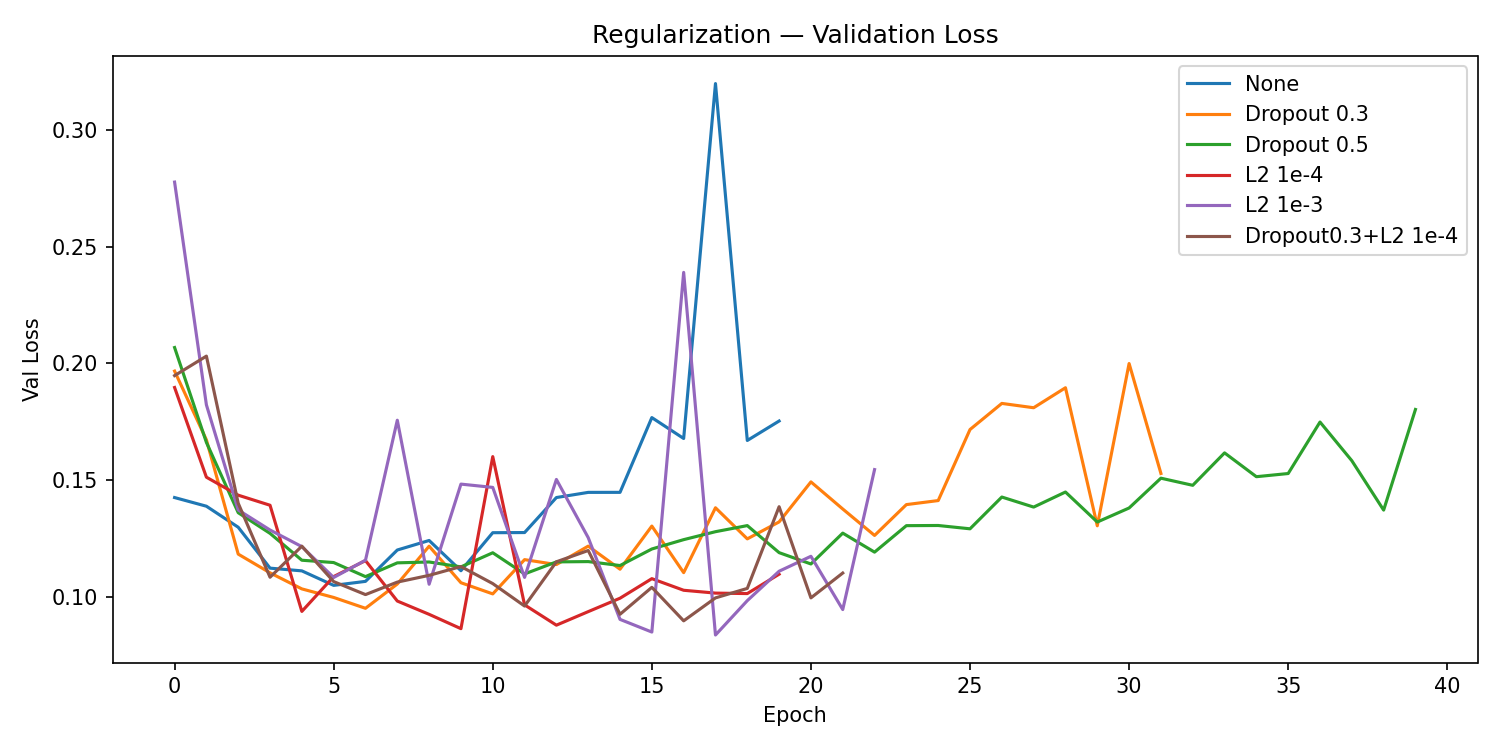
\includegraphics[width=0.85\columnwidth]{reg_curves.png}
  \caption{Validation loss curves for regularisation configurations.}
  \label{fig:reg_curves}
\end{figure}

\subsection{Discussion}
Without regularisation the model shows a train--val gap of 1.54\%,
confirming the overfitting tendency of the large T5 topology.

\textbf{Dropout 0.3} achieves the best validation accuracy (98.26\%)
while reducing the gap to 1.07\%, providing the best
accuracy--generalisation trade-off. It is selected for the final model.

\textbf{Dropout 0.5} reduces the gap further to only 0.42\% (the lowest
of all configurations), but at the cost of 0.1 percentage points of
validation accuracy, as the aggressive masking rate restricts the model's
expressiveness.

\textbf{L2 $\lambda=10^{-4}$} provides only modest regularisation
(gap 1.39\%), as weight decay alone is insufficient to control the
large number of parameters at this penalty strength.

\textbf{L2 $\lambda=10^{-3}$} is too aggressive, reducing train accuracy
notably but yielding the second-lowest validation accuracy (97.33\%) and
the highest variance ($\pm 0.0036$).

\textbf{Combined Dropout 0.3 + L2 $10^{-4}$} produces the second-smallest
gap (0.51\%) but a lower validation accuracy (97.76\%) than Dropout 0.3
alone, suggesting the two regularisers together over-constrain the network.

% ─────────────────────────────────────────────────────────────
\section{Best Model and Final Evaluation}

\subsection{Configuration}

\begin{table}[h]
\centering
\caption{Best model configuration}
\label{tab:best}
\begin{tabular}{ll}
\toprule
Hyperparameter & Value \\
\midrule
Topology        & [2048, 1024, 512, 256, 128] (T5) \\
Optimiser       & RMSprop \\
Learning rate   & 0.001 \\
Activation      & ReLU \\
Dropout         & 0.3 \\
Weight decay    & 0.0 \\
Seeds used      & 42, 123, 456 \\
\bottomrule
\end{tabular}
\end{table}

The final model was retrained from scratch on the combined
train~+~validation set (60\,000 samples) using seed 42 and evaluated on
the 10\,000-sample test set exactly once.

\begin{figure}[h]
  \centering
  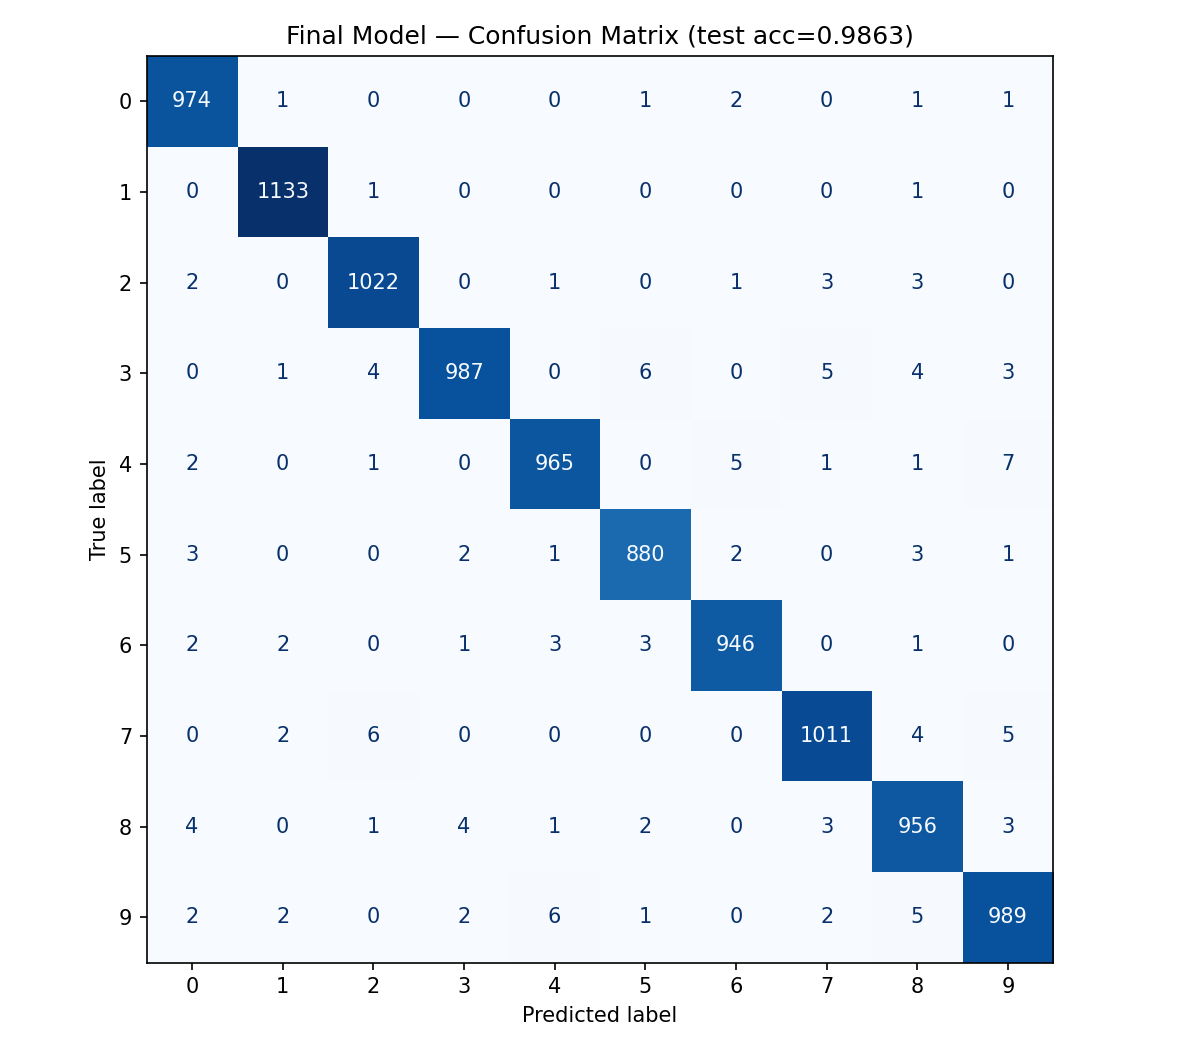
\includegraphics[width=0.85\columnwidth]{final_confusion_matrix.png}
  \caption{Confusion matrix on the test set (test accuracy 98.63\%).}
  \label{fig:cm}
\end{figure}

\begin{table}[h]
\centering
\caption{Final model test accuracy vs baseline}
\label{tab:final}
\begin{tabular}{lr}
\toprule
Model & Test Accuracy \\
\midrule
Logistic Regression (baseline) & 0.9243 \\
Best MLP                       & \textbf{0.9863} \\
\bottomrule
\end{tabular}
\end{table}

The best MLP achieves a test accuracy of \textbf{98.63\%}, a 6.2
percentage-point improvement over the logistic regression baseline
(92.43\%). The confusion matrix (Fig.~\ref{fig:cm}) shows that the most
common errors involve digit pairs that are visually similar (e.g., 4/9
and 3/5).

% ─────────────────────────────────────────────────────────────
\section{Conclusion}

Systematic one-factor-at-a-time hyperparameter tuning on MNIST demonstrates
that each optimisation stage yields meaningful and measurable improvements.
The largest individual gain came from selecting an appropriate topology
(from 97.06\% for T1 to 98.10\% for T5) and choosing an adaptive
optimiser (from 96.80\% for SGD to 98.11\% for RMSprop).
The learning rate of 0.001 proved critical — a tenfold increase to 0.01
caused severe instability, while 0.1 caused complete divergence.
Dropout 0.3 provided the best regularisation, reducing the train--val gap
while boosting validation accuracy by 0.15 percentage points.
All experiments are fully reproducible using seeds 42, 123, and 456 with
a fixed data split generator seed of 42, implemented in
\texttt{Testovanie\_Lobodiuchenko.py}.

% ─────────────────────────────────────────────────────────────
\begin{thebibliography}{1}

\bibitem{lecun1998mnist}
Y.~LeCun, L.~Bottou, Y.~Bengio, and P.~Haffner,
``Gradient-based learning applied to document recognition,''
\emph{Proceedings of the IEEE}, vol.~86, no.~11, pp.~2278--2324, 1998.

\end{thebibliography}

\end{document}
